%%%%%%%%%%%%%%%%%%%%%%%%%%%%%%%%%%%%%%%%%%%%%%%%%%%%%%%%%%%%%%%%%%%%%%%%%%%%%%%%
%2345678901234567890123456789012345678901234567890123456789012345678901234567890
%        1         2         3         4         5         6         7         8

\documentclass[letterpaper, 12 pt, conference]{ieeeconf}  % Comment this line out
                                                          % if you need a4paper
%\documentclass[a4paper, 12pt, conference]{ieeeconf}      % Use this line for a4
                                                          % paper

\IEEEoverridecommandlockouts                              % This command is only
                                                          % needed if you want to
                                                          % use the \thanks command
\overrideIEEEmargins
% See the \addtolength command later in the file to balance the column lengths
% on the last page of the document

\usepackage{hyperref}
\hypersetup{
    colorlinks=true,
    linkcolor=blue,
    filecolor=magenta,      
    urlcolor=cyan,
}

% The following packages can be found on http:\\www.ctan.org
%\usepackage{graphics} % for pdf, bitmapped graphics files
%\usepackage{epsfig} % for postscript graphics files
%\usepackage{mathptmx} % assumes new font selection scheme installed
%\usepackage{times} % assumes new font selection scheme installed
%\usepackage{amsmath} % assumes amsmath package installed
%\usepackage{amssymb}  % assumes amsmath package installed

\title{\LARGE \bf
Programming Assignment 2: Semi-supervised \\Text Classification
}

%\author{ \parbox{3 in}{\centering Narshion Ngao*
%         \thanks{*Use the $\backslash$thanks command to put information here}\\
%         Msc. Computer Systems - 2018\\
%         Jomo Kenyatta University of Agriculture \& Technology \\
%       
%}}

\author{Shihan Ran, A53313589 \\% <-this % stops a space
Fall 2019, CSE 256: Statistical NLP \\
}


% =============== pseudo code package ===============
\usepackage[linesnumbered,ruled,vlined]{algorithm2e}%[ruled,vlined]{
\usepackage{algpseudocode}
\usepackage{amsmath}
\renewcommand{\algorithmicrequire}{\textbf{Input:}}  % Use Input in the format of Algorithm
\renewcommand{\algorithmicensure}{\textbf{Output:}} % Use Output in the format of Algorithm

% =============== figures ===============
\usepackage{graphicx}
\usepackage{subcaption}
\usepackage{mwe}
\usepackage{ulem}

\begin{document}

\maketitle
\thispagestyle{empty}
\pagestyle{empty}

% \input{files/abs.tex}
\section{\textbf{Supervised\\ Improve the Basic Classifier}}

%%%%%%%%%%%%%%%%%%%%%%%%%%%%%%%%%%%%%%%%%%%%%%%%%%%%%%%%%%%%%%%%%%%%%%%%%%%%%%%%
\begin{figure}[!ht]
    \centering
    \begin{subfigure}[b]{0.225\textwidth}
        \centering
        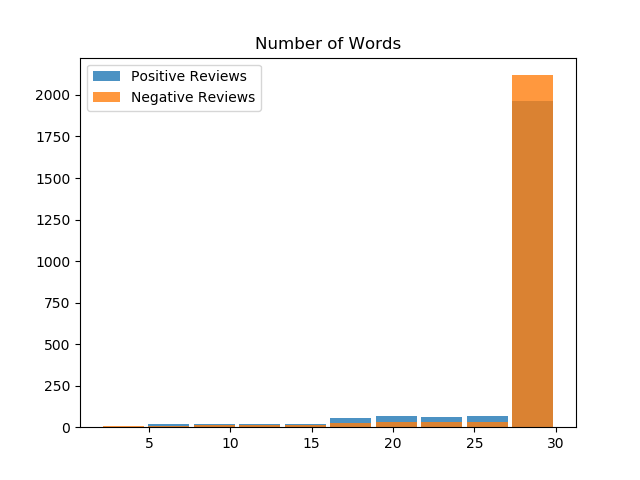
\includegraphics[width=\textwidth]{files/figs/ReviewWord.png}
        \caption[]%
        {{\small Number of Words}}    
        \label{fig:numberofwords}
    \end{subfigure}
    \hfill
    \begin{subfigure}[b]{0.225\textwidth}  
        \centering 
        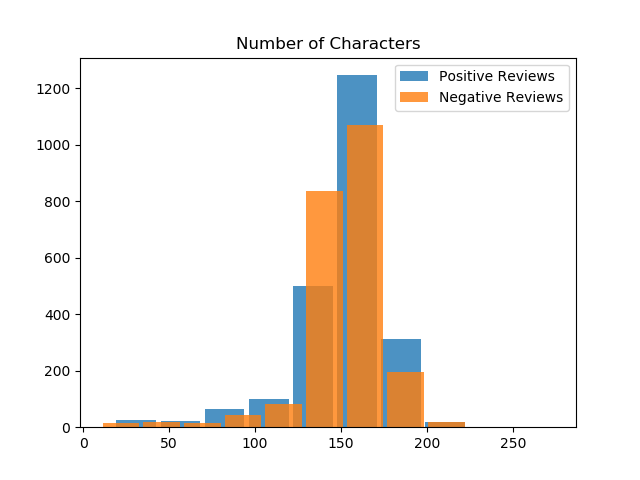
\includegraphics[width=\textwidth]{files/figs/ReviewCharacter.png}
        \caption[]%
        {{\small Number of Characters}}    
        \label{fig:numberofcharacters}
    \end{subfigure}
    \vskip\baselineskip
    \begin{subfigure}[b]{0.225\textwidth}   
        \centering 
        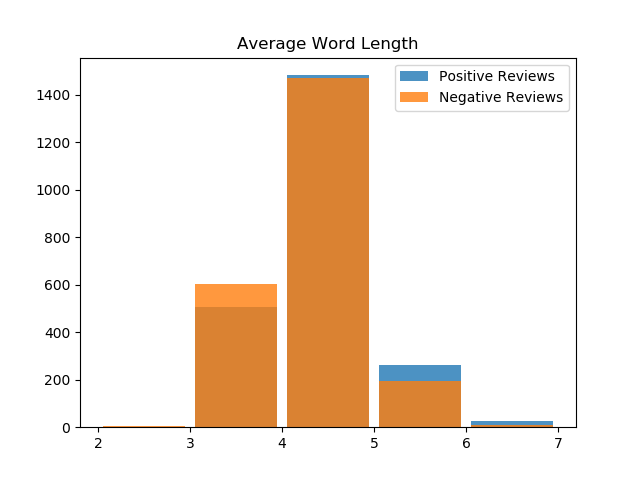
\includegraphics[width=\textwidth]{files/figs/AverageWordLength.png}
        \caption[]%
        {{\small Average Word Length}}    
        \label{fig:averagewordlength}
    \end{subfigure}
    \quad
    \begin{subfigure}[b]{0.225\textwidth}   
        \centering 
        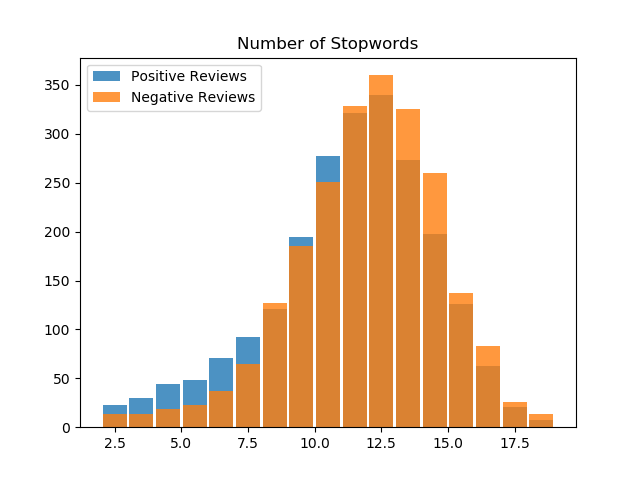
\includegraphics[width=\textwidth]{files/figs/NumberOfStopWords.png}
        \caption[]%
        {{\small Number of Stopwords}}    
        \label{fig:numberofstopwords}
    \end{subfigure}
    \caption[]
    {\small Some basic statistical information about dataset distribution.} 
    \label{fig:distribution}
\end{figure}

\subsection{\textbf{Basis Analysis of Dataset}}

After reading the data set, to perform different tasks on it, we should first perform some basic analysis on the dataset distribution. There are lots of features we can consider, like words, characters, stopwords, special characters, numerics, uppercase words and so on. Here due to limited time and resources, we only select a few indicators to illustrate the problem.

\subsubsection{Number of Words}

One of the most basic functions we can extract from text data is the number of words in each sentence. The intuition behind this is that generally speaking, the negative sentiments should contain a lesser amount of words than the positive ones. 

From figure~\ref{fig:numberofwords}, we can clearly see that due to the reason that sentences are cut off when the word length is longer than 30, there aren't many differences between the distribution of positive reviews and negative reviews.

\subsubsection{Average Word Length}

We also present another feature that will calculate the average word length of each sentence. This can also potentially help us in improving our model. The results are shown in figure~\ref{fig:averagewordlength}.

\subsubsection{Number of Characters}

Generally speaking, when solving a Natural language processing problem, the first thing we should do is preprocessing. The preprocessing can include various operations like spelling correction, tokenization and remove stopwords. Before doing preprocessing, calculating the number of stopwords may give us some extra information that we might have been losing before. The results are shown in figure~\ref{fig:numberofstopwords}.


\subsection{\textbf{Basic Pre-processing}}

Before diving into text and feature extraction, we first clean the training data in order to obtain better features. I tried the following preprocessing steps: transform sentences into lower case, removing punctuations, removing stopwords, common words, and rare words. I also tried different tokenizations. % However, each time I do preprocess, the performances become worse. 

\subsection{\textbf{Feature Engineering}}

Now we have done all the basic preprocessing steps to clean our data. Now, we move on to extract features.

\subsubsection{Term frequency}

Term frequency (TF) is simply the ratio of the count of a word represented in a sentence to the length of the sentence.

\subsubsection{Inverse Document frequency}

The intuition behind inverse document frequency (IDF) is that a word is not of much use if it's occurred in all the sentences. The IDF of each word is the log of the ratio of the total number of sentences to the number of sentences in which that word is present.

\subsubsection{Term frequency - Inverse Document frequency}

TF-IDF is the multiplication of the TF and IDF which we calculated above. TF-IDF can penalize commonly occurring words. We implement this feature using \textit{TfidfVectorizer} from \textit{sklearn.feature\_extraction.text}.

\subsubsection{Bags of Words}

Bag of Words (BoW) refers to the presentation of text which describes the presence of words within the text data. The intuition behind this is that two similar text fields will contain similar kind of words, and will have a similar bag of words. We implement this feature using \textit{CountVectorizer} from \textit{sklearn.feature\_extraction.text}.


\subsection{\textbf{Performances}}

\begin{table}[ht]  %table 里面也可以嵌套tabular,只有tabular是不能加标题的
\centering  %表格居中
\caption{Supervised Performances}
\begin{tabular}{lccc}
\hline
&    \textbf{BoW} & \textbf{BoW+TFIDF} & \textbf{BoW+TFIDF+Tuned \textit{LR}}\\
\hline
 \textbf{Train}   & 0.9997 &  0.9860 &  \textbf{1.0}   \\
 \textbf{Dev} &  0.7795 &  0.7773  &  \textbf{0.7948}   \\
\hline
\end{tabular}
\label{tab:supervised}
\end{table}

We created a model pipeline and performed an exhaustive hyperparameter search using \textit{GridSearchCV} from \textit{sklearn.model\_selection}. Some of the performances can be found in figure~\ref{fig:hyper}.

\begin{figure}[!ht]
    \centering
    \begin{subfigure}[]{0.225\textwidth}
        \centering
        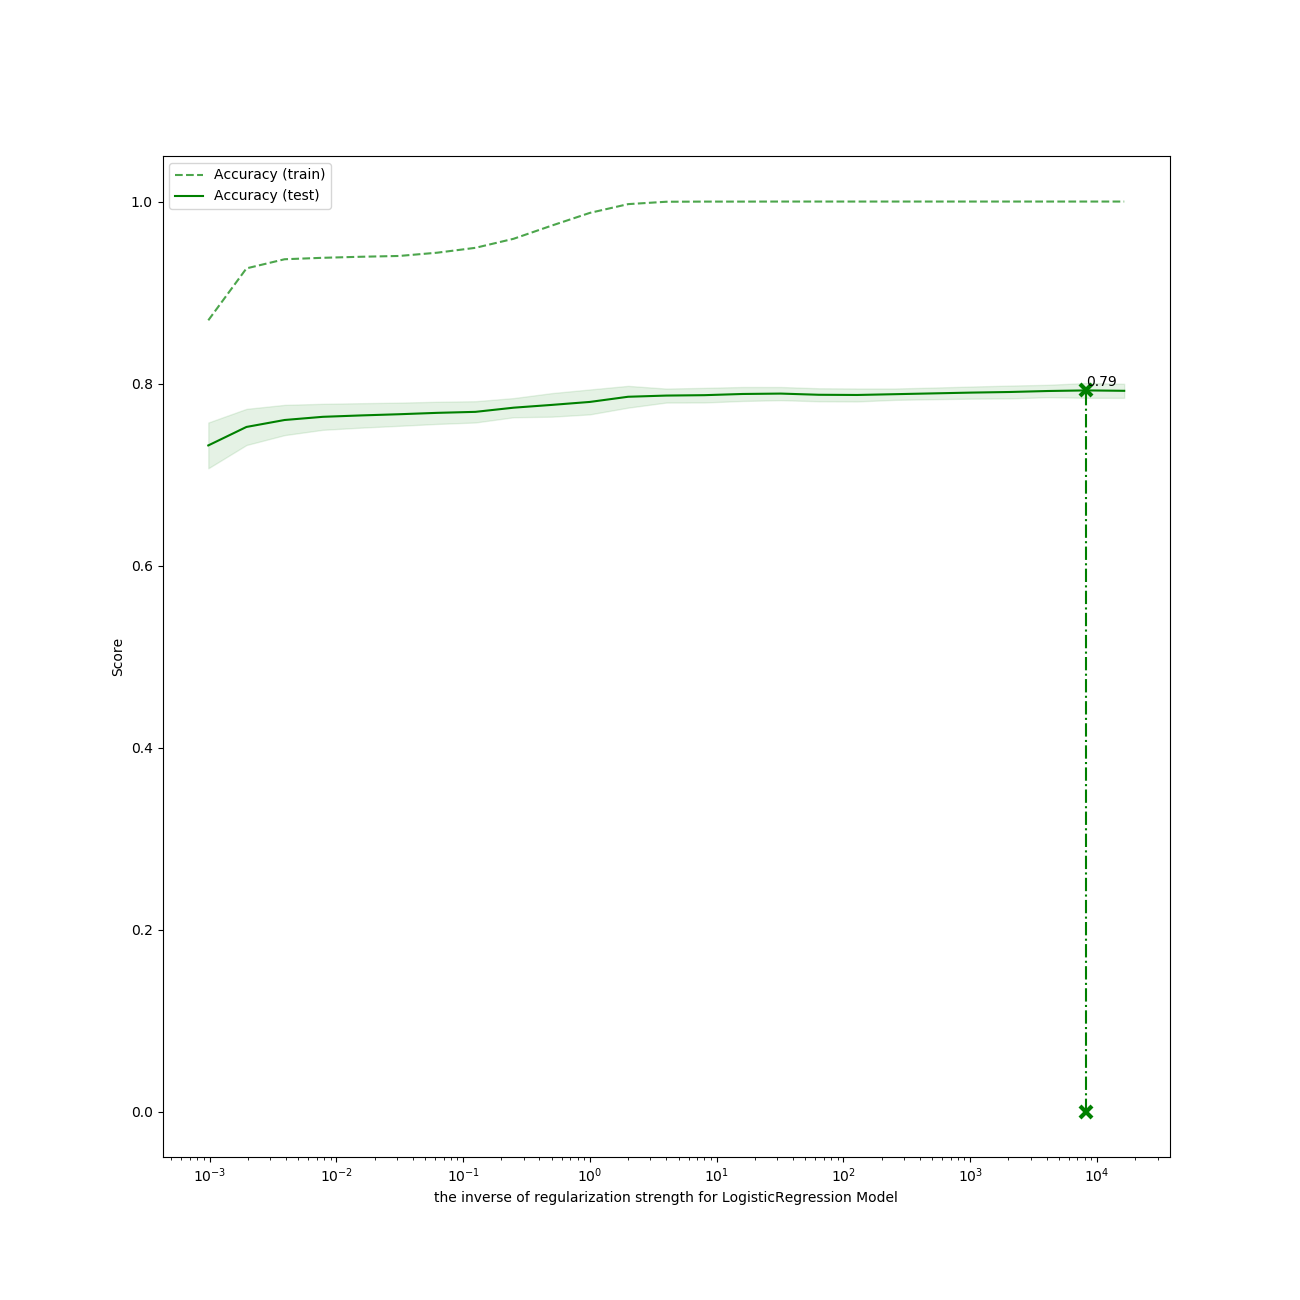
\includegraphics[width=\textwidth]{files/figs/finetuneC.png}
        \caption[]%
        {{\small Fine-tuned on regularization strength}}    
        \label{fig:numberofwords}
    \end{subfigure}
    % \hfill
    \begin{subfigure}[]{0.225\textwidth}  
        \centering 
        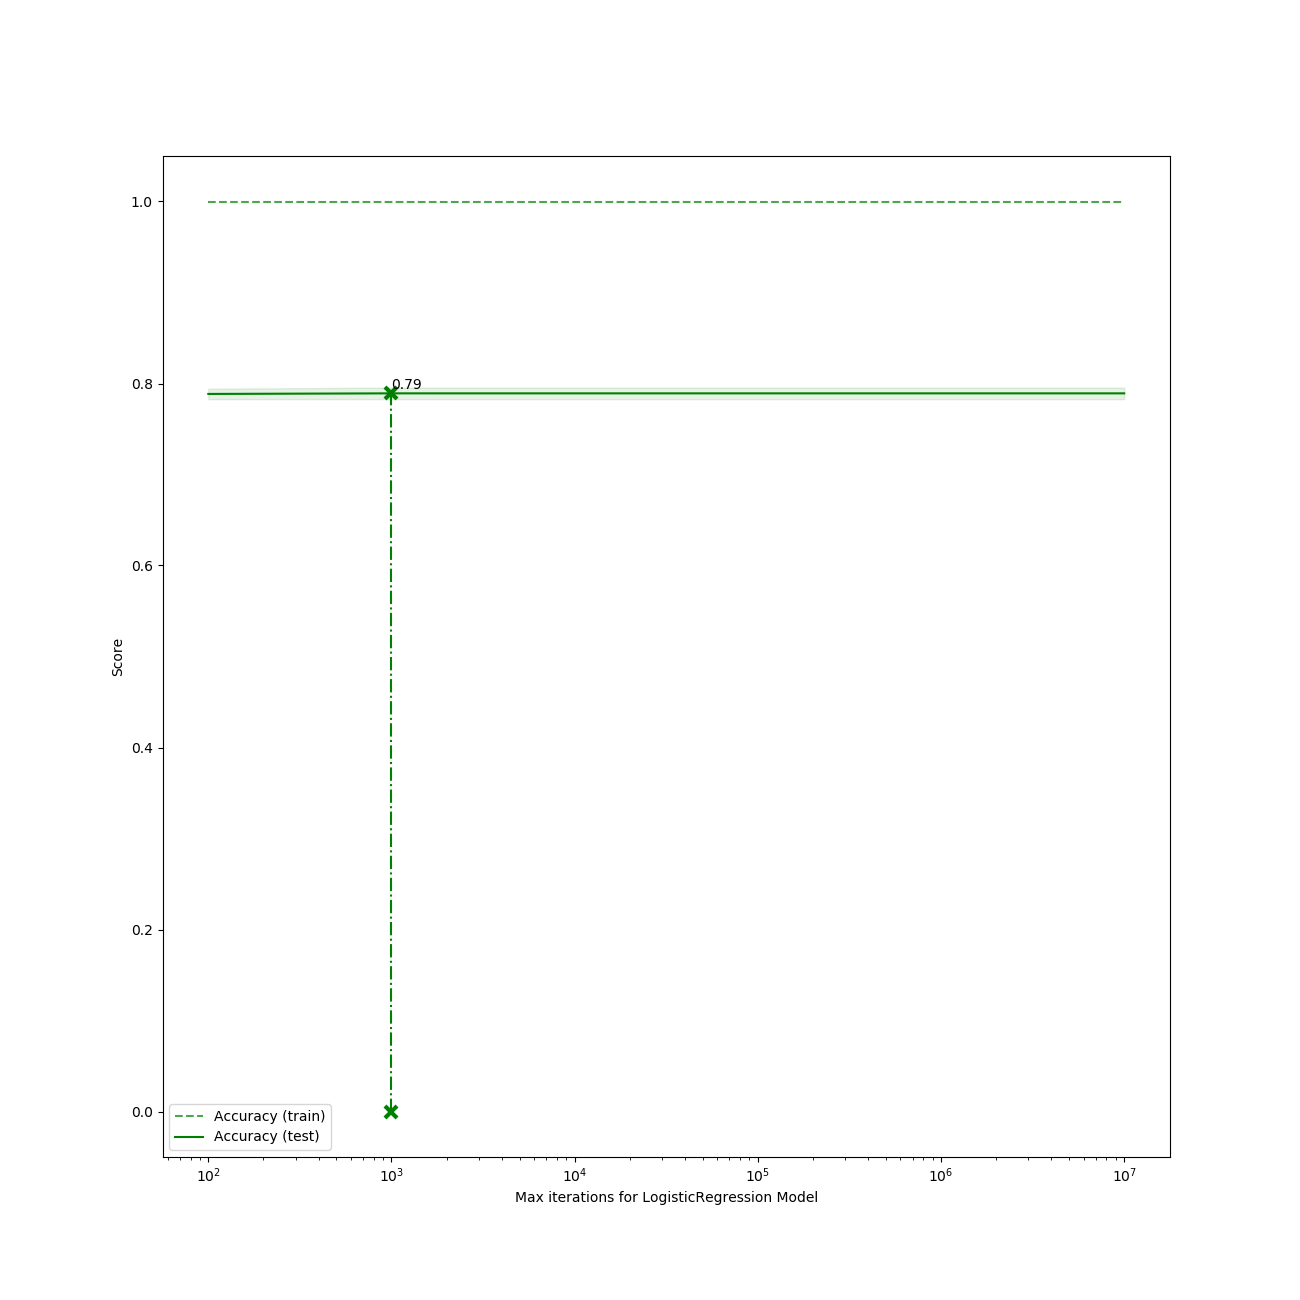
\includegraphics[width=\textwidth]{files/figs/finetuneIterations.png}
        \caption[]%
        {{\small Fine-tuned on max iterations}}
        \label{fig:numberofcharacters}
    \end{subfigure}
    \caption[]
    {\small Model performances on different hyperparameter settings.} 
    \label{fig:hyper}
\end{figure}

\begin{table}[ht]  %table 里面也可以嵌套tabular,只有tabular是不能加标题的
\centering  %表格居中
\caption{HyperParameters}
\begin{tabular}{lc}
\hline
&    \textbf{Parameters}\\
\hline
 \textbf{\textit{CountVectorizer}}   & \textit{max/min\_df, ngram\_range, stop\_words} \\
 \textbf{\textit{TfidfVectorizer}} &  \textit{use\_idf, smooth\_idf, sublinear\_tf} \\
 \textbf{\textit{LogisticRegression}} &  \textit{C, solver, max\_iter, class\_weight} \\
\hline
\end{tabular}
\label{tab:supervised}
\end{table}

The best performances were acheived under
\begin{itemize}
\item \textit{ngram\_range=(1,3)}
\item \textit{use\_idf=True}, \textit{smooth\_idf=False}
\item \textit{C=512}, \textit{solver='saga'}, \textit{max\_iter=1000}
\item DO NOT use any preprocess
\item DO NOT remove stopwords
\end{itemize}

From our experiments, we know that features from count-based vectorization methods like BoW and TF-IDF have some disadvantages:

\begin{enumerate}
\item They describe sentences by word occurrences while completely ignoring the relative position information of the words in the sentence (despite using N-grams, which is only a quick fix). 
\item TF-IDF word vectors are usually very high dimensional.
\item They are not able to capture semantics.
\end{enumerate}



\section{\textbf{Semi-supervised\\ Exploiting Unlabeled Data}}

%%%%%%%%%%%%%%%%%%%%%%%%%%%%%%%%%%%%%%%%%%%%%%%%%%%%%%%%%%%%%%%%%%%%%%%%%%%%%%%%
\subsection{\textbf{The approach to utilize unlabeled data}}

My approach to semi-supervised learning is to iteratively expand the labeled data and retrain the classifier.

\begin{algorithm}[]
  \caption{Semi-Supervised}
  \KwIn{$D_{u}$ as unlabeled data, $D_{l}$ as labeled data, $ratio$, $threshold$}
  \KwOut{Model parameters $\theta$}
  $\hat{D}_l \leftarrow D_l, \hat{D}_u \leftarrow D_u$\;
  \While{$\hat{D}_u > (1-ratio)*D_u$}
  {
    $\theta \leftarrow \text{Train}(\hat{D}_l)$\;
    $D'_u \leftarrow \text{Predict}(\theta, \hat{D}_u)$\;
    $\hat{D}_l \leftarrow \text{Expand}(\hat{D}_l, D'_u, threshold)$\;
    $\hat{D}_u \leftarrow \text{Remove}(D'_u, threshold)$\;
  }
  return $\theta$\;
\end{algorithm}

The first thing is to decide which labels to include in $\hat{D}_l$ in every iteration. We choose to include the most confident predictions (i.e., the probability of these predictions should be bigger than the $threshold$).

The second thing is to decide the stopping criterion. Instead of choosing a fixed number of iterations, we choose to stop when a certain $ratio$ of $D_u$ has been added into the labeled training data $\hat{D}_l$.

In order to make our performances better, We tried different combinations of $ratio$ and $threshold$.

\subsection{\textbf{The effect of size of labeled data}}

Usually, larger datasets can help us avoid over-fitting. If our model has many parameters and it isn't fed enough data, then it will tend to memorize the training set and perform poorly on the dev/test set. To avoid this phenomenon, except for using special training techniques like regularization, we can also use a semi-supervised method. By using semi-supervised learning, it is possible to combine the advantages of working with a smaller labeled dataset to guide the learning process and a larger unlabeled dataset to increase the generalizability of the solution. 

In order to make it possible for semi-supervised learning methods to make the most of the labeled and unlabeled data, some assumptions are needed for the underlying structure of data space. The labeled and unlabeled data points should share the same data space. If the distributions are hugely different for those two data, then adding labeled data may and confuse our model and thus decrease our performances.

\subsection{\textbf{Features and changes}}

There should exist an overlapping between the unlabeled data and labeled data. When adding those unlabeled data into our training data, we will augment those overlapped words. Whether using BoW or TF-IDF, the features of overlapped words will change enormously, which will further lead to the result that their weights may change significantly. 

Meanwhile, for those not overlapped words, while their features may remain the same, it can be regarded as their weights decreases.

\subsection{\textbf{Performances}}

We can refer to figure~\ref{fig:threshold} to see the performances of $Ratio=0.7$ on different thresholds. Overall speaking, compared with supervised learning, the performances on development set is decreasing as we add more labeled data to our training sets. 

\begin{figure}[!ht]
    \centering
    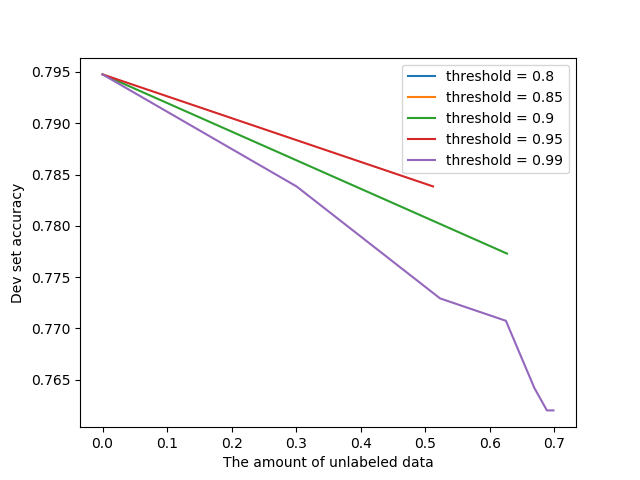
\includegraphics[width=0.45\textwidth]{files/figs/semi.png}
    \caption[]%
    {{\small Performances of Ratio=0.7 on different thresholds}}
    \label{fig:threshold}
\end{figure}

The first thing we should notice is our model can achieve a high accuracy of about 0.8 on the development set and  1.0 on the training set. Thus, our threshold should be bigger than 0.8.

What we should know is that the unlabeled data is so noisy and it even contains some Chinese and Japanese words. If not selected precisely, adding those data as labeled data may confuse your model and decrease the accuracy.

When the threshold is low, each iteration we will have more confident data and thus can add more labeled data into our training data. So after two or three iterations then we will achieve the stopping criterion since the amount of unlabeled data is larger than our ratio. However, a lower threshold means you are less confident about the precision of your prediction. As the threshold increases, each iteration will get a smaller amount of confident data. Thus, we will need more iterations. The higher threshold should mean the prediction is more accurate. There is a tradeoff between the precision and the number of iterations. 

\subsection{\textbf{Error Analysis on semi-supervised classifier}}

I sampled the following sentences and their respective labels generated by supervised learning and semi-supervised learning. 

\begin{itemize}
\item \textit{"This is a serious matter that needs to be addressed.. I've had my fair share of chipotle, and this one by far is the most stingiest.. Us Fat ass American's".} Supervised Model labeL: Negative. Semi-Supervised Model Label: Positive. Ground Truth: Negative.
\item \textit{'Went there for the first time last night to celebrate a friends birthday.  OMG!  The porkchops were unbelievable. Met the owner, Eddie.  Good friends, great food'} Supervised Model labeL: Negative. Semi-Supervised Model Label: Positive. Ground Truth: Positive.
\end{itemize}

\begin{table}[ht]  %table 里面也可以嵌套tabular,只有tabular是不能加标题的
\centering  %表格居中
\caption{Statistical Information}
\begin{tabular}{lccc}
\hline
&    \textbf{Train} & \textbf{Dev} & \textbf{Unlabeled} \\
\hline
 \textbf{Total} & 4582 & 458 & 91524 \\
 \textbf{Positive}   & 2291 &  229 &  -   \\
 \textbf{Negative} &  2291 &  229  &  -  \\
\hline
\end{tabular}
\label{tab:stat}
\end{table}

\begin{table}[ht]  %table 里面也可以嵌套tabular,只有tabular是不能加标题的
\centering  %表格居中
\caption{Labels for Unlabeled data}
\begin{tabular}{lcc}
\hline
&    \textbf{Supervised Model} & \textbf{Semi-Supervised Model}  \\
\hline
 \textbf{Total} & 91524 & 91524  \\
 \textbf{Positive}   & 44202 &  43325 \\
 \textbf{Negative} & 47322  &  48199  \\
\hline
\end{tabular}
\label{tab:unlabel}
\end{table}

We can see from Table~\ref{tab:stat} that the original dataset is pretty balanced. It contains the same number of positive samples and negative samples.

However, according to Table~\ref{tab:unlabel}, the distribution of our predicted label isn't like the original one. The semi-supervised model tends to predict more negative labels than the supervised model. There are 4331 different labels out of 91524 lines in the prediction from our two models.








\section{\textbf{Semi-supervised\\ Designing better Features}}

\subsection{\textbf{Define better features}}

Our goal is to utilize the unlabeled corpus to learn something about the word semantics and use it to identify the words that are likely to indicate the same sentiment.

We choose word2vec. Word2vec is a model that embeds words in a lower-dimensional vector space using a shallow neural network. The result is a set of word-vectors where vectors close together in vector space have similar meanings based on context, and word-vectors distant to each other have differing meanings. There are two versions of this model based on skip-gram and continuous-bag-of-words. 

\subsection{\textbf{Performances}}

We use the word embedding trained on our unlabeled text corpus as our features. Since our unlabeled data isn't big enough, we do a hyperparameter tuning on the dimension of word embedding. The results are shown in Table~\ref{tab:dimen}. Bigger size values require more training data and training time, but can lead to a better and more accurate model.

\begin{table}[ht]  %table 里面也可以嵌套tabular,只有tabular是不能加标题的
\centering  %表格居中
\caption{Performances on different dimensions of the trained word embedding}
\begin{tabular}{lcccc}
\hline
&    \textbf{50} & \textbf{100} & \textbf{150} & \textbf{200} \\
\hline
 \textbf{Train} & 0.643 & 0.655 & 0.657 & 0.658\\
 \textbf{Dev}   & 0.659 & \textbf{0.670} & 0.668 & 0.666\\
\hline
\end{tabular}
\label{tab:dimen}
\end{table}

Overall, the performances of only using word embedding features is worse than our previous supervised model.
\section{\textbf{Kaggle}}

User name: shihanran

Display name: Shihan Ran

Email: sran@ucsd.edu

\begin{thebibliography}{99}

\bibitem{c1} Robin Tommy, Gullapudi Sundeep and Hima Jose, 2017. Automatic Detection and Correction of Vulnerabilities using Machine Learning.
\bibitem{c2} Sanjay Kumar, Ari Viinikaineny and Timo Hamalainenz, 2016. Machine Learning Classification Model For Network Based Intrusion Detection System
\bibitem{c3} Gauri Kalnoor and Jayashree Agarkhed, 2016. Preventing Attacks and Detecting Intruder for Secured Wireless Sensor Networks.
\bibitem{c4} Hsiu-Chuan Huang, Zhi-Kai Zhang, Hao-Wen Cheng, and Shiuhpyng Winston Shieh, 2017. Web Application Security: Threats, Countermeasures, and Pitfalls


\end{thebibliography}

\end{document}
